\section{pbdR}

\hidenum
\begin{frame}[noframenumbering]
\frametitle{Contents}
 \tableofcontents[currentsection,hideothersubsections,sectionstyle=show/hide]
\end{frame}
\shownum

\subsection{Problems with R}

\begin{frame}
%  \addtocounter{framenumber}{-1}
  \begin{block}{Problems with R}\pause
  We \emph{love} R!  However\dots
  \begin{itemize}[<+-|alert@+>]
    \item Slow.
    \item If you don't know what you're doing, it's \emph{really} slow.
    \item Performance improvements usually for small machines.
    \item Very ram intensive.
    \item Chokes on big data.
  \end{itemize}
  \end{block}
\end{frame}

\begin{frame}
%  \addtocounter{framenumber}{-1}
  \begin{block}{Problems with R: Big Data}\pause
  One of R's biggest problems is an indexing limitation:
  \begin{itemize}[<+-|alert@+>]
    \item Any one R object must (at present) be indexed by a 32-bit integer.
    \item Largest vector/matrix:  16gb
    \item Largest square matrix:  $46340\times 46340$
  \end{itemize}
  \end{block}
\end{frame}

\begin{frame}[shrink]
  \begin{block}{R and Parallelism}
    The solution to many of R's problems is parallelism.  However \dots\vspace{-.4cm}
   \begin{center}
    \begin{minipage}[t]{.95\textwidth}
    \begin{block}{\centering What we have}
      \begin{enumerate}[<+-|alert@+>]
	\item Mostly serial.
	\item Parallelism mostly not distributed.
	\item Data parallelism mostly explicit.
      \end{enumerate}
    \end{block}
    \end{minipage}
    \\\pause
    \begin{minipage}[t]{.95\textwidth}
    \begin{block}{\centering What we want}
      \begin{enumerate}[<+-|alert@+>]
        \item Mostly parallel.
        \item Mostly distributed.
        \item Mostly implicit.
      \end{enumerate}
    \end{block}
    \end{minipage}
    \end{center}
    \end{block}
\end{frame}


\subsection{The pbdR Project}

\begin{frame}[squeeze]
  \begin{block}{Programming with Big Data in R (pbdR)}\pause
  Goals:  \emph{Productivity, Portability, Performance}\\[.4cm]\pause
  Our Approach:
  \begin{itemize}[<+-|alert@+>]
    \item Series of \emph{free}\footnote{MPL, BSD, and GPL licensed} R packages.
    \item Scalable, big data analytics with high-level syntax.
    \item Implicit management of distributed data details.
    \item Methods have syntax \emph{identical} to R.
    \item Powered by state of the art numerical libraries (MPI, ScaLAPACK, PBLAS, BLACS, LAPACK, BLAS, \dots)
  \end{itemize}
  \end{block}
\end{frame}

\begin{frame}[shrink]
  \begin{block}{pbdR Packages}
    \begin{center}
	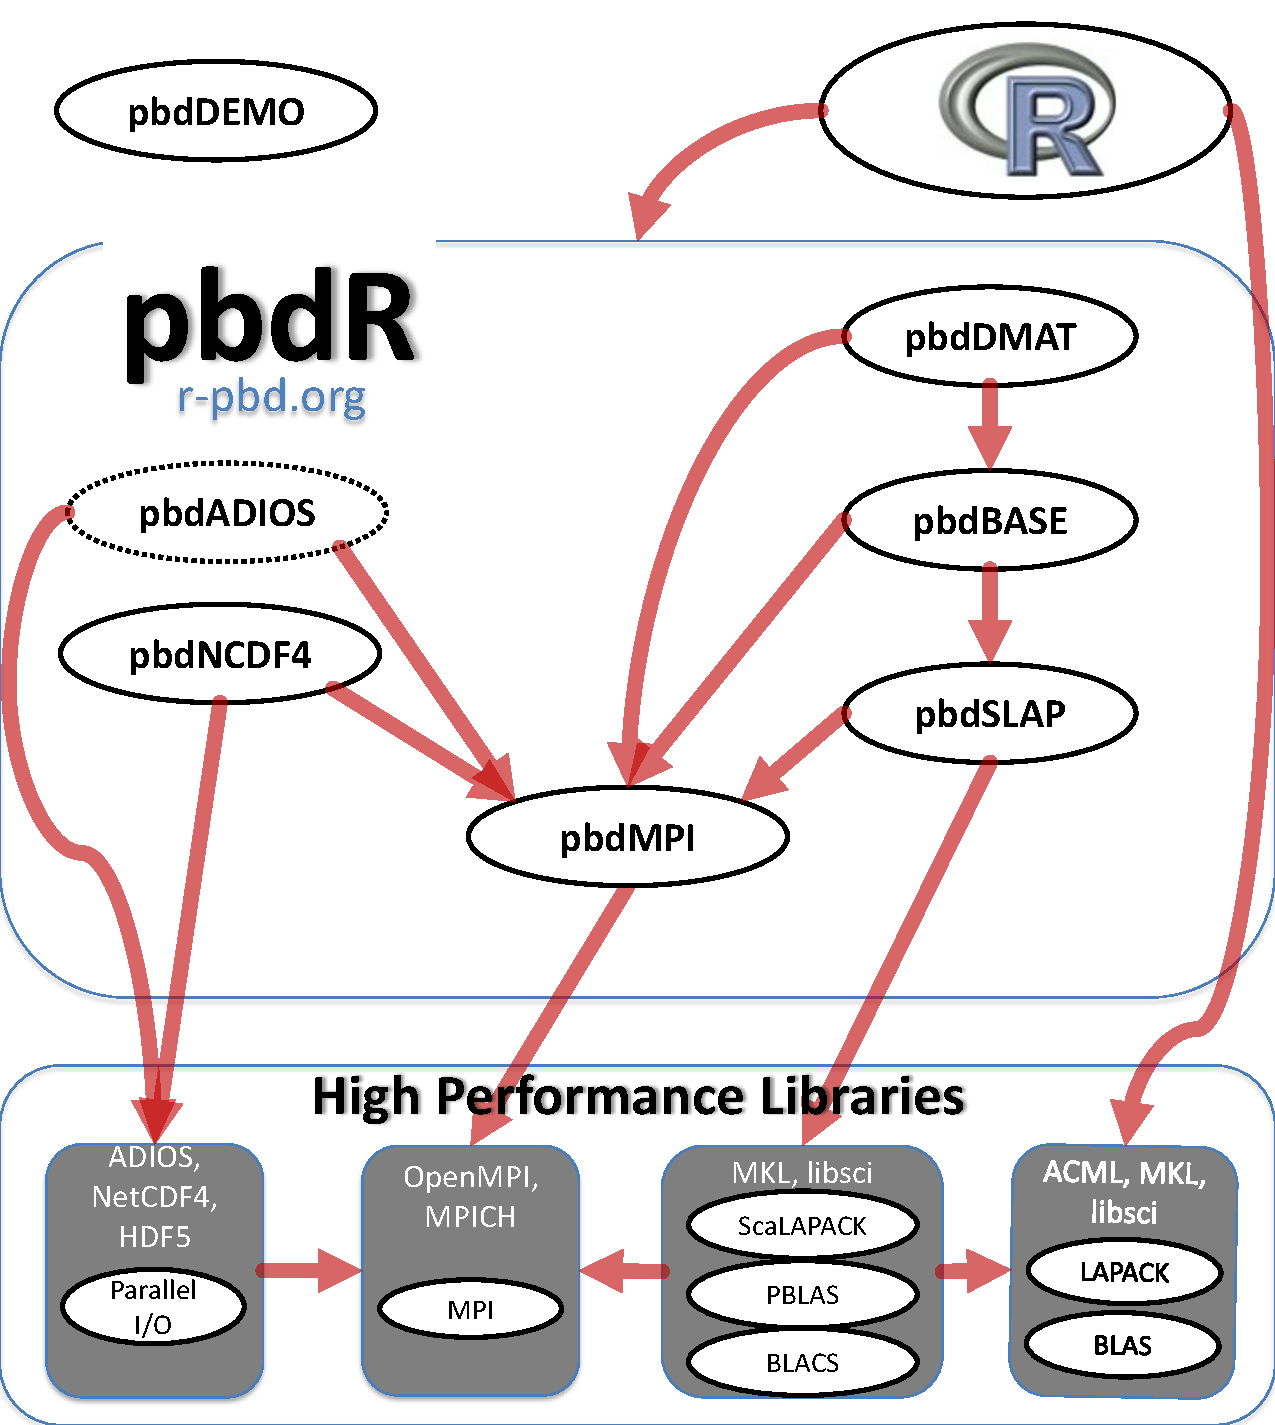
\includegraphics[width=7cm, height=7cm]{pics/pbdpacks}
    \end{center}
  \end{block}
\end{frame}


\begin{frame}[shrink]
  \begin{block}{pbdR Packages --- http://code.r-pbd.org}\pause
  Released to CRAN:
  \begin{itemize}[<+-|alert@+>]
    \item \pkg{pbdMPI}: MPI bindings (explicit, low-level)
    \item \pkg{pbdSLAP}: Foreign library (just install it, nothing to use)
    \item \pkg{pbdBASE}: Compiled code (used by DMAT, also for devs)
    \item \pkg{pbdDMAT}: Distributed matrices (mostly implicit, high-level)
    \item \pkg{pbdNCDF4}: Parallel NetCDF4 reader
    \item \pkg{pbdDEMO}: Package demonstrations, examples, vignette written in textbook style
  \end{itemize}
%     \\[.2cm]
    Future Development:
  \begin{itemize}[<+-|alert@+>]
    \item \pkg{pbdADIOS}: Wrappers for ADIOS middleware
    \item Profiling tools
    \item Client/server interface for interactive sessions
    \item Something for you\dots?
  \end{itemize}
  \end{block}
\end{frame}

\begin{frame}
  \begin{block}{SPMD}\pause
  The pbdR Packages enable high-level ``Single Program/Multiple Data'' (SPMD) programming:
    \begin{itemize}
      \item SPMD is a programming \emph{paradigm}.
      \item Arguably the simplest extension of serial programming.
      \item Sort of like trying to explain breathing \dots
      \item Not to be confused with SIMD.
      \item SPMD utilizes MIMD architecture computers.
      \item Only one program is written, executed in batch independently on all processors.
      \item Different processors are autonomous; there is no manager.
%       \item Like ``Map/Reduce'', you probably used it without knowing it even had a name.
    \end{itemize}
  \end{block}
\end{frame}


\begin{frame}[fragile]
  \begin{block}{SPMD}\pause
      SPMD codes are run in batch (non-interactively):
\begin{lstlisting}[backgroundcolor=\color{white},keywordstyle=\color{black},title=From the Shell]
mpirun -np 4 Rscript my_script.R
\end{lstlisting}
  \end{block}
\end{frame}


\begin{frame}[fragile]
  \begin{block}{Example Syntax}\pause
  \begin{lstlisting}
x <- x[-1, 2:5]
xtx <- t(x) %*% x
ans <- svd(solve(xtx))
  \end{lstlisting}
  \begin{center}
  \pause Look familiar?\\[.4cm] \pause
  \emph{The above runs on 1 core with R or 10,000 cores with pbdR}
  \end{center}
  \end{block}
\end{frame}



\subsection{Installing pbdR}

\begin{frame}[fragile]
  \begin{block}{Installation}\pause
  Installing pbdR is about as easy as possible, and generally amounts to:
  \begin{lstlisting}
install.packages(pbdMPI)
install.packages(pbdNCDF4)
install.packages(pbdSLAP)
install.packages(pbdBASE)
install.packages(pbdDMAT)
install.packages(pbdDEMO)
  \end{lstlisting}
  But this assumes you have MPI installed on your system\dots
  \end{block}
\end{frame}


\begin{frame}[fragile]
  \begin{block}{NICS Allocation}\pause
  Instead, consider getting an allocation on Nautilus:
  \begin{center}
  \url{http://www.nics.tennessee.edu/getting-an-allocation}\\
  
\includegraphics[scale=.3]{pics/nics}
  \end{center}
  \end{block}
\end{frame}